
\documentclass{report}

\usepackage[utf8]{inputenc}
\usepackage[italian]{babel}
\usepackage{import}
\usepackage{todonotes}
\usepackage{color}
\usepackage{rotating}
\usepackage[hidelinks]{hyperref}
\usepackage{url}
\usepackage{pdfpages}
\usepackage{siunitx}
\usepackage{pdflscape}
\usepackage{subfig}
\usepackage[euler]{textgreek}
\usepackage{mhchem}

\usepackage{enumerate} 
\usepackage{amsmath}
\usepackage{amsfonts}

\usepackage[signatures,swapnames,sans]{frontespizio}

\usepackage{geometry}
\geometry{portrait, margin=3cm}
\usepackage{siunitx}
\usepackage{booktabs}

\renewcommand*\figurename{Figura}

\newcommand{\sub}[1]{\textsubscript{#1}}
\newcommand{\super}[1]{\textsuperscript{#1}}
\newcommand{\parallelsum}{\mathbin{\!/\mkern-5mu/\!}}

\newcommand{\Fig}[0]{Fig.}

\usepackage{titlesec}

\titleformat{\chapter}{\normalfont\huge}{}{20pt}{\huge\bfseries}

\linespread{1.3}

\begin{document}
\addtocounter{chapter}{+5}
	\begin{frontespizio}
		\Margini{3cm}{3cm}{3cm}{3cm}
		\Universita{Bergamo}
		\Logo[43.332mm]{unibg-mark}
		\Divisione{Scuola di Ingegneria}
		\Corso[Laurea Magistrale]{Ingegneria Informatica}
		\Titolo{Laboratorio di Elettronica}
		\Sottotitolo{Relazione progetto circuito}
		\Punteggiatura{}
		\NRelatore{Prof.}{Prof.}
		\Relatore{Luigi Gaioni}
		\Candidato[1058231]{Giulia Allievi}
		\Candidato[1059640]{Martina Fanton}
		\Annoaccademico{2022--2023}
		\begin{Preambolo*}
			\usepackage[italian]{babel}
			\usepackage[T1]{fontenc}
			\usepackage[utf8]{inputenc}
			\usepackage{microtype}
			\usepackage{lmodern}
			\graphicspath{{img/}}
			
			\renewcommand{\frontinstitutionfont}{\fontsize{14}{17}\bfseries\scshape}
			\renewcommand{\fronttitlefont}{\fontsize{17}{21}\bfseries\scshape}
			\renewcommand{\frontfootfont}{\fontsize{12}{14}\bfseries\scshape}
		\end{Preambolo*}
	\end{frontespizio}

%----------------------------------------------------------------------------------------
%	PAGINA BIANCA
%----------------------------------------------------------------------------------------
\newpage
\null
\thispagestyle{empty}
\newpage

\chapter{Relazione progetto circuito}
\section*{Introduzione}
Il progetto richiede di realizzare un circuito che, superata una temperatura di riferimento, generi un allarme luminoso lampeggiante. Il sistema deve essere automatico, reversibile e realizzato hardware, senza avere a disposizione microcontrollori. Si hanno a disposizione:
\begin{itemize}
\item un termistore NTC;
\item un LED rosso;
\item un comparatore;
\item un timer 555;
\item componenti passivi.
\end{itemize}
La temperatura di riferimento è \SI{25}{\celsius}, a questa temperatura la resistenza del termistore NTC è di \SI{1}{k\ohm}.
% modifica per non copiare da slide ? 

\newpage
\section{Progettazione del circuito}
Per progettare il circuito, progetteremo e dimensioneremo separatamente la rete del termistore e la rete oscillante, quindi integreremo le sue sottoreti per ottenere il progetto del sistema finale.
\subsection{Progettazione della rete oscillante}
Inizialmente progettiamo la rete oscillante. Configuriamo il timer 555 in modo tale che funzioni in modalità astabile. Lo schema scelto è mostrato in figura \ref{figura:schema555}, i pin sono collegati in questo modo:
\begin{itemize}
\item PIN 1, è il terminale di \textit{ground}, perciò è collegato a massa;
\item PIN 2, è il terminale di \textit{trigger}, è cortocircuitato con il PIN 6;
\item PIN 3, è l'\textit{uscita}, a cui sarà collegato il LED tramite una resistenza;
\item PIN 4, è il terminale di \textit{reset}, servirà per gestire il collegamento alla rete che pilota il termistore;
\item PIN 5, è il terminale di \textit{control voltage}, non lo utilizziamo, è collegato a massa tramite una capacità di filtraggio ($\mathrm{C_1}$);
\item PIN 6, è il terminale di \textit{threshold}, gestisce la carica della capacità $\mathrm{C_2}$ attraverso la resistenza $\mathrm{R_1}$;
\item PIN 7, è il terminale di \textit{discharge}, pilota la scarica della capacità $\mathrm{C_2}$ attraverso la resistenza $\mathrm{R_2}$;
\item PIN 8, è il terminale di \textit{alimentazione}. 
\end{itemize} 
Tra i pin 6 e 7 viene collegato un diodo (l'anodo è collegato al pin 7 mentre il catodo al pin 6), la sua funzione è quella di bypassare la resistenza $\mathrm{R_2}$ nella fase di carica del condensatore, in modo tale da ottenere un oscillatore con duty cycle variabile da 0\% a 100\%. 
\begin{figure}[h!]
	\centering
	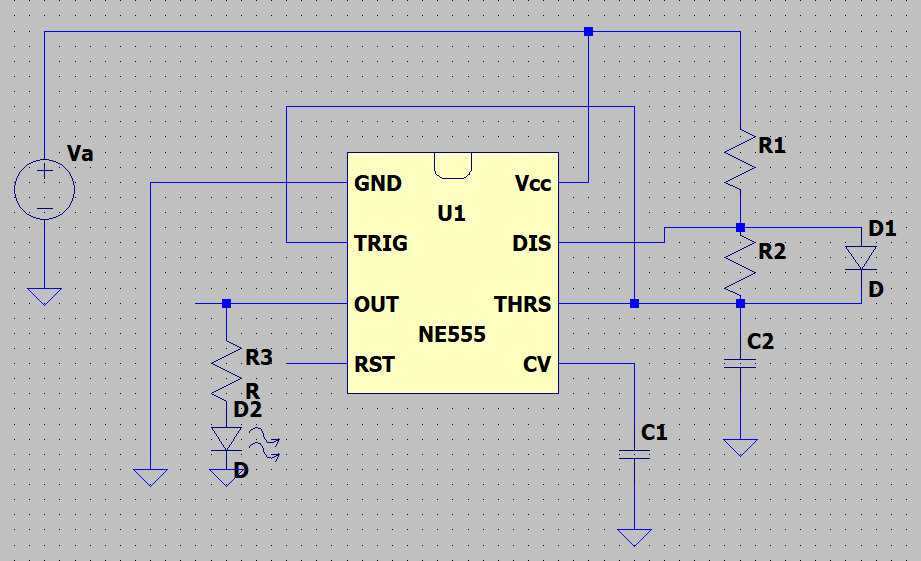
\includegraphics[height=6.9cm]{immagini/schema555}
	\caption{Schema della rete oscillante.} 
	\label{figura:schema555}
\end{figure}
\\Successivamente, dimensioniamo la rete oscillante. Le grandezze da dimensionare sono:
\begin{itemize}
\item tensione di alimentazione $V_A$;
\item capacità $C_1$ e $C_2$;
\item resistenze $R_1$, $R_2$ e $R_3$.
\end{itemize}
Per primo, scegliamo il valore che deve avere la tensione di alimentazione $V_A$. Dal \textcolor{blue}{\underline{\href{https://www.ti.com/lit/ds/symlink/lm555.pdf?ts=1667144089940&ref_url=https\%253A\%252F\%252Fwww.ti.com\%252Fproduct\%252FLM555}{datasheet}}} del timer 555, vediamo che il componente deve essere alimentato con una tensione compresa fra \SI{4.5}{\volt} e \SI{16}{\volt}: dato che il progetto della rete del termistore (sezione \ref{rete_termistore}) prevederà di utilizzare un OPAMP, scegliamo un valore compatibile anche con questo componente, in modo tale da avere un'unica tensione di alimentazione per il circuito finale. Dal \textcolor{blue}{\underline{\href{https://www.ti.com/lit/ds/symlink/ua741.pdf?ts=1672216941275&ref_url=https\%253A\%252F\%252Fwww.ti.com\%252Fproduct\%252FUA741}{datasheet}}} del \textmu A741, un amplificatore operazionale \textit{general purpose}, sappiamo che dobbiamo scegliere una tensione duale o singola compresa fra \SI{-18}{\volt} e +\SI{18}{\volt}. Di conseguenza, dobbiamo scegliere un valore di  $V_A$ di circa \SI{10}{\volt}: visto che nella realtà il circuito non funzionerà con un alimentatore da banco, ma con delle batterie, scegliamo di alimentare i componenti attivi con una tensione da \SI{9}{\volt}, così da poter utilizzare queste batterie. \par
Successivamente, scegliamo i valori delle capacità. La capacità $\mathrm{C_1}$ serve per filtrare il segnale di massa da eventuali disturbi, il valore consigliato dal datasheet è di \SI{0.01}{\mu\farad}, perciò $\displaystyle{C_1=\SI{0.01}{\mu\farad}}$. La capacità $\mathrm{C_2}$ regola il periodo di oscillazione, scegliamo una capacità da \SI{200}{\mu\farad}. \par
Dimensionate le capacità, scegliamo i valori che devono avere le resistenze $R_1$ e $R_2$. Per fare ciò, decidiamo prima per quanto tempo il LED deve rimanere acceso e per quanto spento, da questi due intervalli di tempo ricaveremo i valori delle due resistenze. Le formule che descrivono queste due grandezze sono:
\\$$t_{low}=\ln2\cdot R_2\cdot C_2\indent\indent\indent \mathrm{e}\indent\indent\indent t_{high}=\ln2\cdot R_1\cdot C_2$$
Vorremmo che il LED resti spento per \SI{1}{\second} e acceso per \SI{2}{\second}, dunque $\displaystyle{t_{low}=\SI{1}{\second}}$ e $\displaystyle{t_{high}=\SI{2}{\second}}$. Perciò, dalle formule inverse si ricavano i valori delle resistenze $R_1$ e $R_2$:
\\$$R_2 = \frac{t_{low}}{\ln2\cdot C_2}=\frac{\SI{1}{\second}}{0.693\cdot\SI{200}{\mu\farad}}=\SI{7.213}{k\ohm}\simeq\SI{7.5}{k\ohm}$$
$$R_1 = \frac{t_{high}}{\ln2\cdot C_2}=\frac{\SI{2}{\second}}{0.693\cdot\SI{200}{\mu\farad}}=\SI{14.427}{k\ohm}\simeq\SI{15}{k\ohm}$$
Con i valori delle resistenze approssimati ai valori reali, i due tempi risultano $\displaystyle{t_{low}=\SI{1.04}{\second}\mathrm{\;e\;}t_{high}=\SI{2.08}{\second}}$, perciò i calcoli risultano in accordo con quanto scelto. \par
L'ultima resistenza da dimensionare è $\mathrm{R_3}$. Questa resistenza ha lo scopo di ridurre la corrente che fluisce nel LED, altrimenti si rischia di bruciarlo. Di solito, in questi dispositivi circola una corrente di 15\SI{-20}{m\ampere}, per il dimensionamento ipotizziamo che nel diodo circoli una corrente pari a \SI{20}{m\ampere}, mentre la caduta di tensione ai capi di un LED di colore rosso è di \SI{1.8}{\volt}. Per ricavare il valore di $\mathrm{R_3}$, basta utilizzare la legge di Ohm:
$$\indent i_R = i_D\indent\rightarrow\indent \frac{V_{out}-V_D}{R_3}=i_D\indent\rightarrow\indent\frac{\SI{9}{\volt}-\SI{1.8}{\volt}}{R_3}=\SI{20}{m\ampere}$$
$$\Rightarrow\indent R_3=\frac{(9\SI{-1.8}{)\volt}}{\SI{20}{m\ampere}}=\SI{360}{\ohm}$$
Per $\mathrm{R_3}$ scegliamo una resistenza da \SI{500}{\ohm}, di conseguenza nel diodo fluirà una corrente di circa \SI{15}{m\ampere}. \par 
Nell'immagine in figura \ref{figura:dim555} è mostrato il sottosistema della rete oscillante con i valori scelti per ogni componente. 
\begin{figure}[h!]
	\centering
	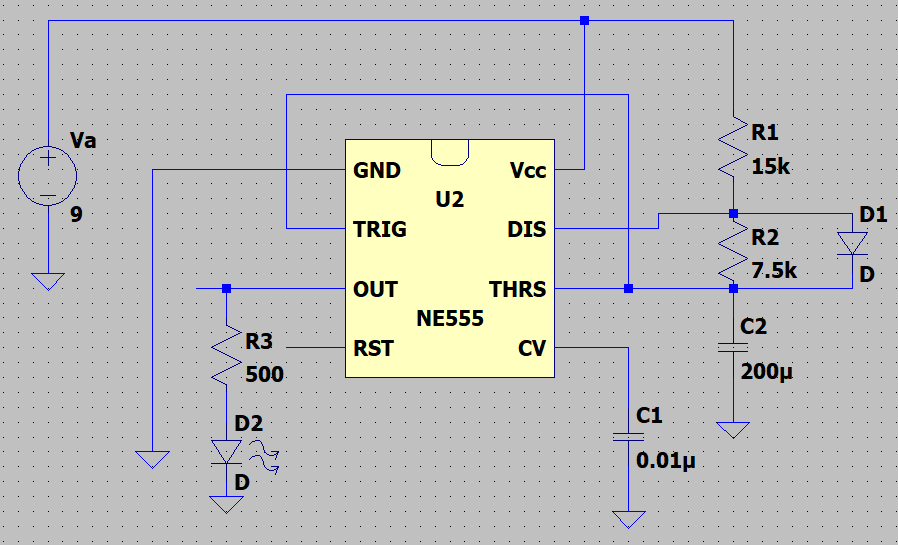
\includegraphics[height=6.9cm]{immagini/dim555}
	\caption{Schema della rete oscillante dimensionata.} 
	\label{figura:dim555}
\end{figure}
\\Nella figura \ref{figura:555out} vengono invece mostrati i grafici che si ottengono in uscita (corrente che fluisce nel LED e tensione ai suoi capi) quando il circuito si trova nello stato di allarme e di riposo. \par
\begin{figure}[h!]
	\centering
	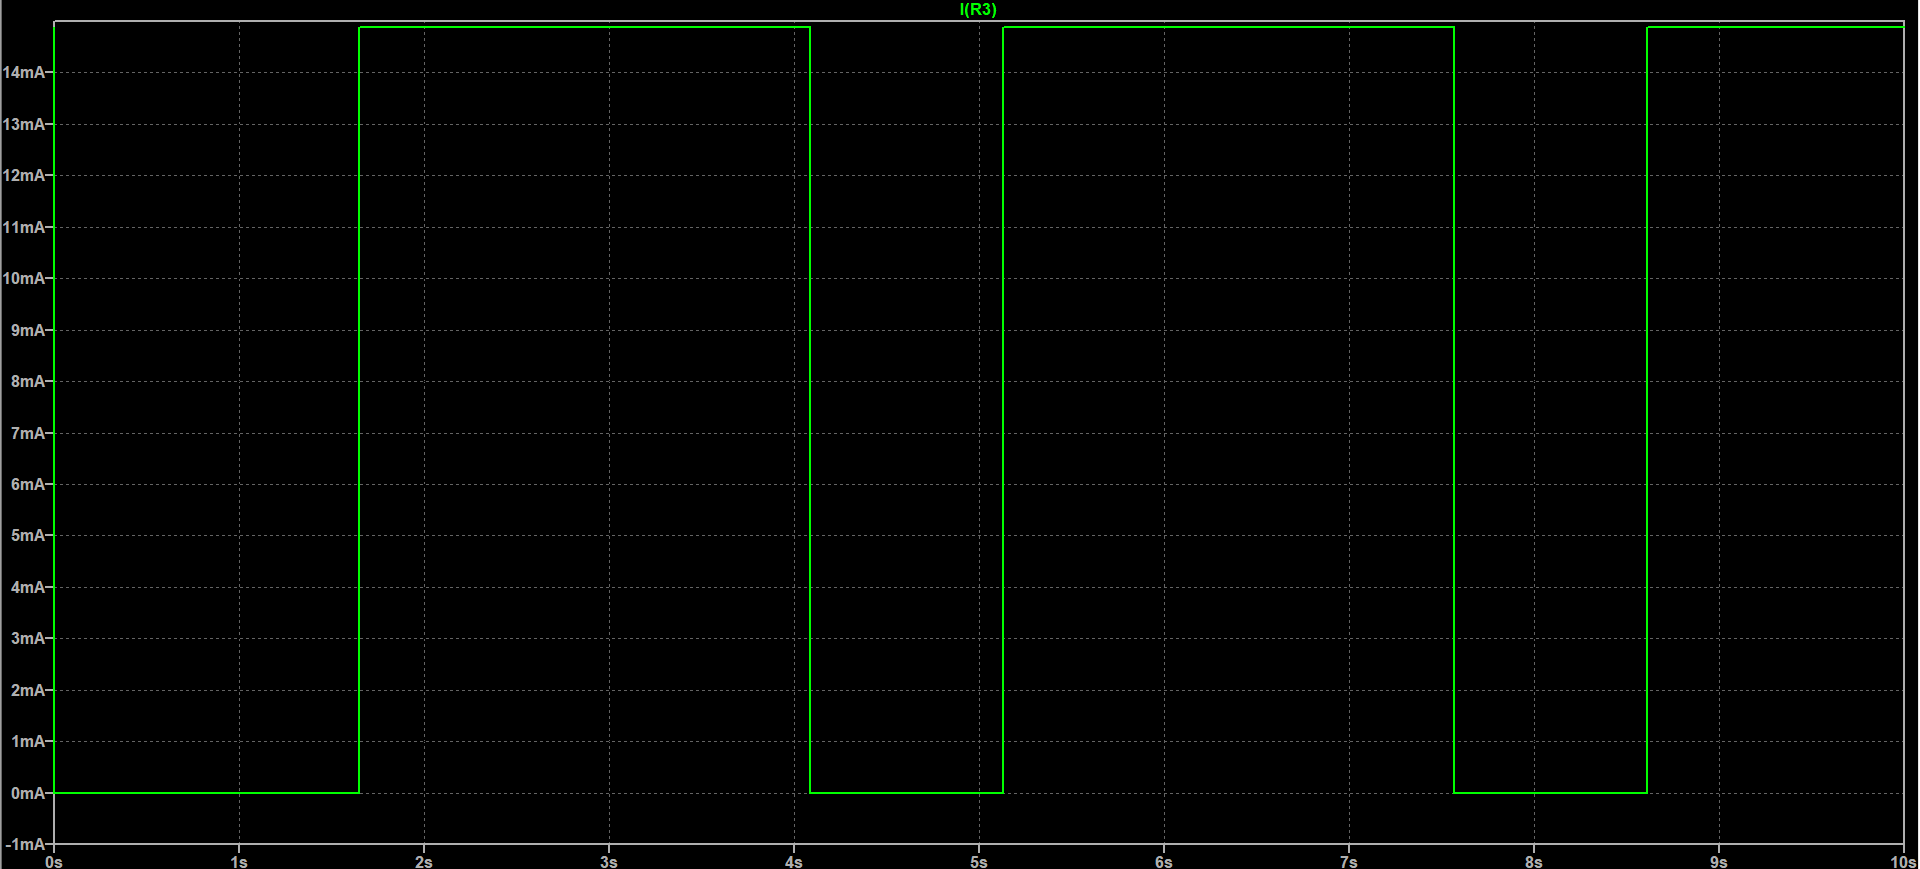
\includegraphics[height=6cm]{immagini/555on}
	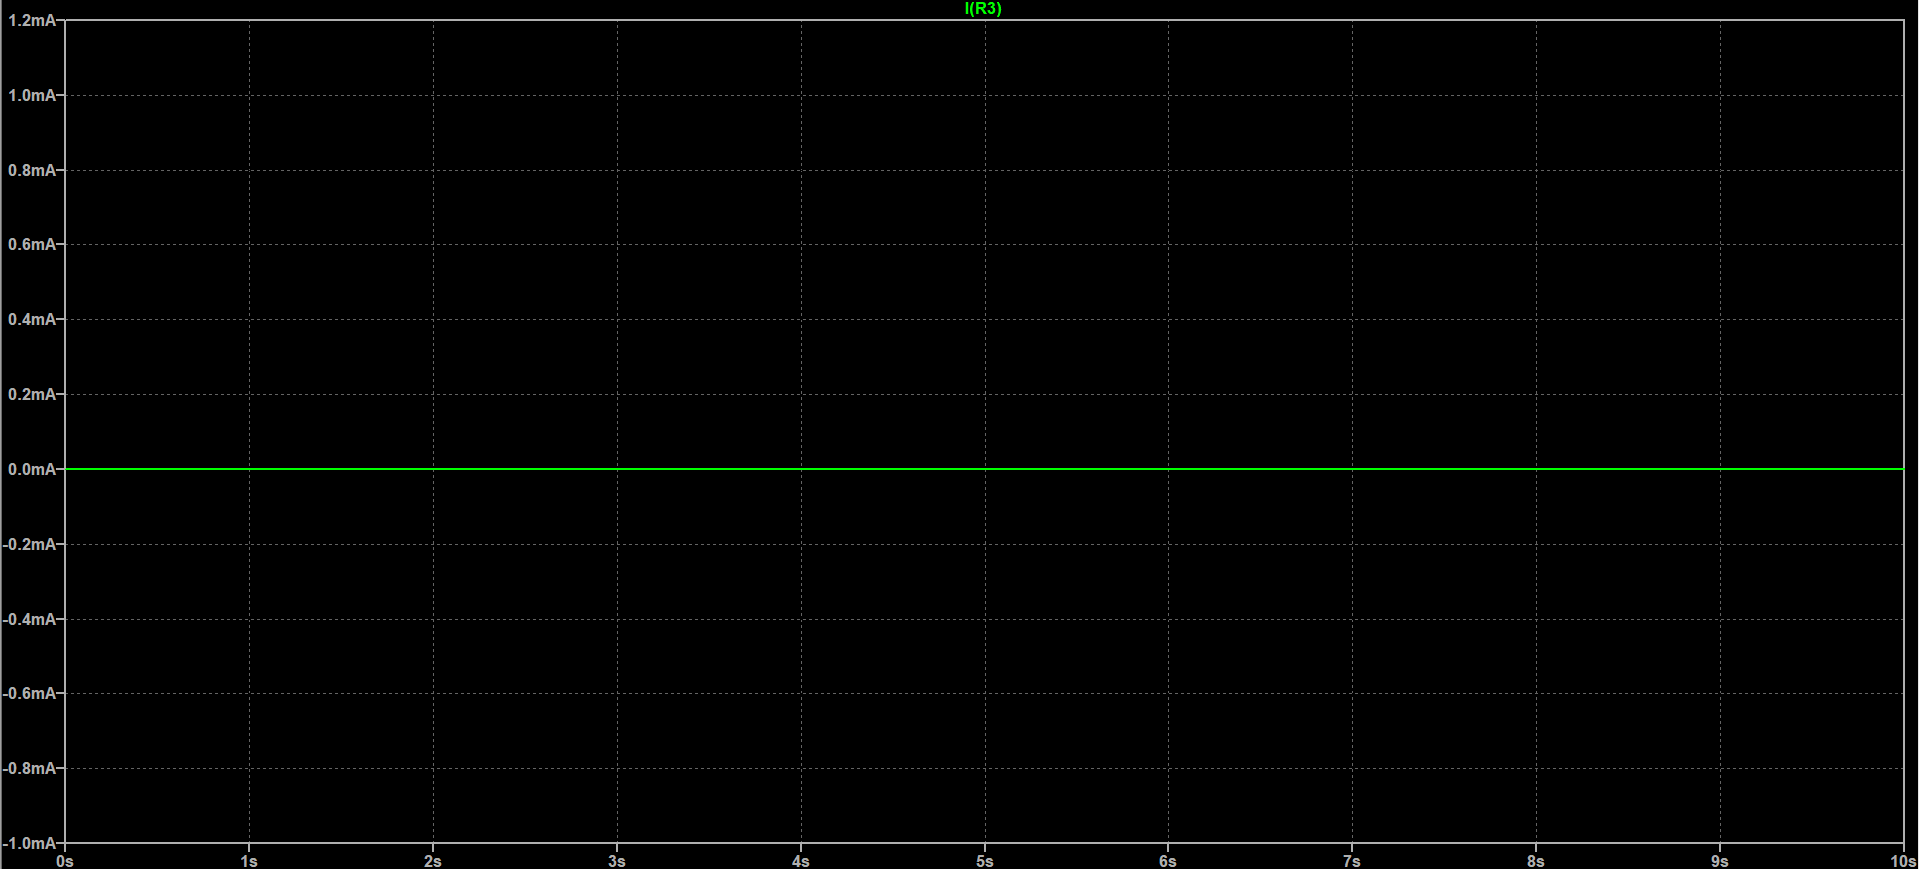
\includegraphics[height=6cm]{immagini/555off}
	\caption{Grafico dell'uscita quando il sistema è nello stato di allarme (sopra) e riposo (sotto).} 
	\label{figura:555out}
\end{figure}
Nel primo caso, la temperatura sarà superiore a \SI{25}{\celsius}, quindi il sistema si troverà nello stato di allerta. Il circuito si comporterà come un oscillatore, perciò, terminato il transitorio iniziale, l'uscita resta alta per circa due secondi e bassa per circa un secondo. Le imprecisioni su $t_{high}$ sono dovute al fatto che nei calcoli è stata trascurata la caduta di tensione data dal diodo D1, perciò quest'intervallo di tempo è di poco superiore rispetto a quanto dimensionato. Dalle misure con i cursori, questa differenza risulta essere pari a \SI{0.36}{\second}. \par
Nel secondo caso invece, il sistema registrerà una temperatura inferiore a \SI{25}{\celsius}, di conseguenza nel LED non deve fluire corrente perché deve rimanere spento, dato che il sistema non è nello stato di allarme.
\subsection{Progettazione della rete del termistore}\label{rete_termistore}
Per gestire le due situazioni descritte alla fine della sezione precedente, dobbiamo pilotare opportunamente il pin 4, ovvero il \textit{reset}, del timer 555. In particolare, se la temperatura è inferiore a \SI{25}{\celsius}, sul pin 4 deve essere applicato un segnale di tensione che corrisponde al livello logico basso (\SI{0}{\volt}), perché vogliamo che anche l'uscita si trovi al livello logico basso in modo tale che il LED non si accenda. Al contrario, se la temperatura è superiore alla temperatura di riferimento, al reset deve essere applicato un segnale corrispondente al livello logico alto (\SI{9}{\volt}), così da far lavorare il timer 555 in modalità astabile e pilotare l'accensione e lo spegnimento del LED secondo i tempi scelti nella sezione precedente. Queste scelte sono dovute al fatto che il timer 555 viene resettato quando si applica un impulso negativo sul pin 4 (fonte: \textcolor{blue}{\underline{\href{https://www.ti.com/lit/ds/symlink/lm555.pdf?ts=1667144089940&ref_url=https\%253A\%252F\%252Fwww.ti.com\%252Fproduct\%252FLM555}{datasheet}}}), e questa transizione la otteniamo se utilizziamo le tensioni come appena descritto. \par
Il segnale che pilota il reset è dato dall'OPAMP, che sarà utilizzato in configurazione di comparatore: per la nostra applicazione, è necessario configurare gli ingressi invertente e non invertente per fare in modo che la condizione $V^+>V^-$ si verifichi quando la temperatura è superiore a \SI{25}{\celsius}, così che l'uscita dell'amplificatore operazionale sia alta; il viceversa deve invece verificarsi quando la temperatura è minore del valore critico. Inoltre, per ottenere in uscita i segnali descritti al paragrafo precedente, dovremo alimentare l'OPAMP con una tensione singola, cioè fra massa e $V_A$. \par
Per decidere come dimensionare gli ingressi, dobbiamo prima capire il comportamento elettrico del termistore al variare della temperatura. Un termistore NTC è schematizzabile come una resistenza variabile, il cui andamento in funzione della temperatura (in kelvin) è di tipo esponenziale:
$$ R_T = R_0\cdot e^{B\bigl(\frac{1}{T}-\frac{1}{T_0}\bigr)}$$
Dalla specifica, sappiamo che $R_0$ vale \SI{1}{k\ohm} quando $T_0 = \SI{25}{\celsius}=\SI{298}{\kelvin}$. Il parametro $B$ varia in base al termistore scelto e in particolare per un termistore NTC con le nostre caratteristiche vale circa \SI{3000}{\kelvin}, come possiamo ricavare dal \textcolor{blue}{\underline{\href{https://www.mouser.it/datasheet/2/240/Littelfuse_Leaded_Thermistors_Glass_Encapsulated_T-1315924.pdf}{datasheet}}}. Sostituendo alla relazione precedente le grandezze note, otteniamo:
$$R_T = 42.45\cdot 10^{-3}\;\SI{}{\ohm}\cdot e^{\bigl(\frac{\SI{3000}{\kelvin}}{T}\bigr)} $$
Dalla formula, verifichiamo che a \SI{25}{\celsius} la resistenza è effettivamente di \SI{1}{k\ohm}. Sempre da questa formula, ci aspettiamo che se la temperatura aumenta, la resistenza $\mathrm{R_T}$ diminuisce; viceversa, se la temperatura diminuisce, questa resistenza aumenta. Infatti, se calcoliamo la resistenza per due valori di temperatura, uno maggiore e l'altro minore di \SI{25}{\celsius} (= \SI{298}{\kelvin}), otteniamo:
$$R_{T=\SI{283}{\kelvin}} = 42.45\cdot 10^{-3}\;\SI{}{\ohm}\cdot e^{\bigl(\frac{\SI{3000}{\kelvin}}{\SI{283}{\kelvin}}\bigr)}=\SI{1.70}{k\ohm}>\SI{1}{k\ohm}\indent\mathrm{per \;}T = \SI{10}{\celsius}=\SI{283}{\kelvin}$$
$$R_{T=\SI{313}{\kelvin}} = 42.45\cdot 10^{-3}\;\SI{}{\ohm}\cdot e^{\bigl(\frac{\SI{3000}{\kelvin}}{\SI{313}{\kelvin}}\bigr)}=\SI{617}{\ohm}<\SI{1}{k\ohm}\;\;\;\indent\mathrm{per \;}T = \SI{40}{\celsius}=\SI{313}{\kelvin}$$
Nella fase di simulazione del circuito, utilizzeremo questi due valori per analizzare le due diverse situazioni. \par
Agli ingressi dell'operazionale, possiamo utilizzare due partitori, di cui uno formato da due resistenze da \SI{1}{k\ohm}, mentre l'altro da una resistenza da \SI{1}{k\ohm} e dal termistore NTC. La tensione in uscita al primo partitore è fissa e pari a:
$$V_1 = \frac{\SI{1}{k\ohm}}{\SI{1}{k\ohm}+\SI{1}{k\ohm}}\cdot V_A = \frac{V_A}{2} = \SI{4.5}{\volt}$$
L'uscita del secondo partitore è invece funzione di $R_T$. La resistenza da \SI{1}{k\ohm} la colleghiamo fra l'uscita del partitore e massa, mentre il termistore NTC fra l'alimentazione e l'uscita del partitore, pertanto la tensione in uscita vale:
$$V_2 = \frac{\SI{1}{k\ohm}}{R_T+\SI{1}{k\ohm}}\cdot V_A$$
In particolare, se $R_T>\SI{1}{k\ohm}$ (ovvero $T<\SI{25}{\celsius}$), allora $V_2<V_A/2\;$; viceversa se $R_T<\SI{1}{k\ohm}$ (ossia $T>\SI{25}{\celsius}$), allora $V_2>V_A/2$. Sfruttando questi due partitori in ingresso all'OPAMP, possiamo confrontare una tensione che è funzione della temperatura con una tensione fissa che corrisponde alla soglia dei \SI{25}{\celsius} e produrre un'uscita diversa in base al fatto che la temperatura sia maggiore o minore di questo riferimento. \par
Terminato il dimensionamento dei due partitori, dobbiamo decidere quale collegare all'ingresso invertente e quale all'ingresso non invertente. Ricordando che la condizione $V^+>V^-$ deve verificarsi quando la temperatura è superiore a \SI{25}{\celsius}, e sapendo che se la temperatura è superiore a \SI{25}{\celsius}, $V_2$ è maggiore di $V_A/2$, allora $V_1=V^-$ e $V_2=V^+$. Di conseguenza, il primo partitore sarà collegato all'ingresso invertente, mentre il secondo all'ingresso non invertente. Lo schema complessivo della rete del termistore è rappresentato in figura \ref{figura:dimNTC}. \par
\begin{figure}[h!]
	\centering
	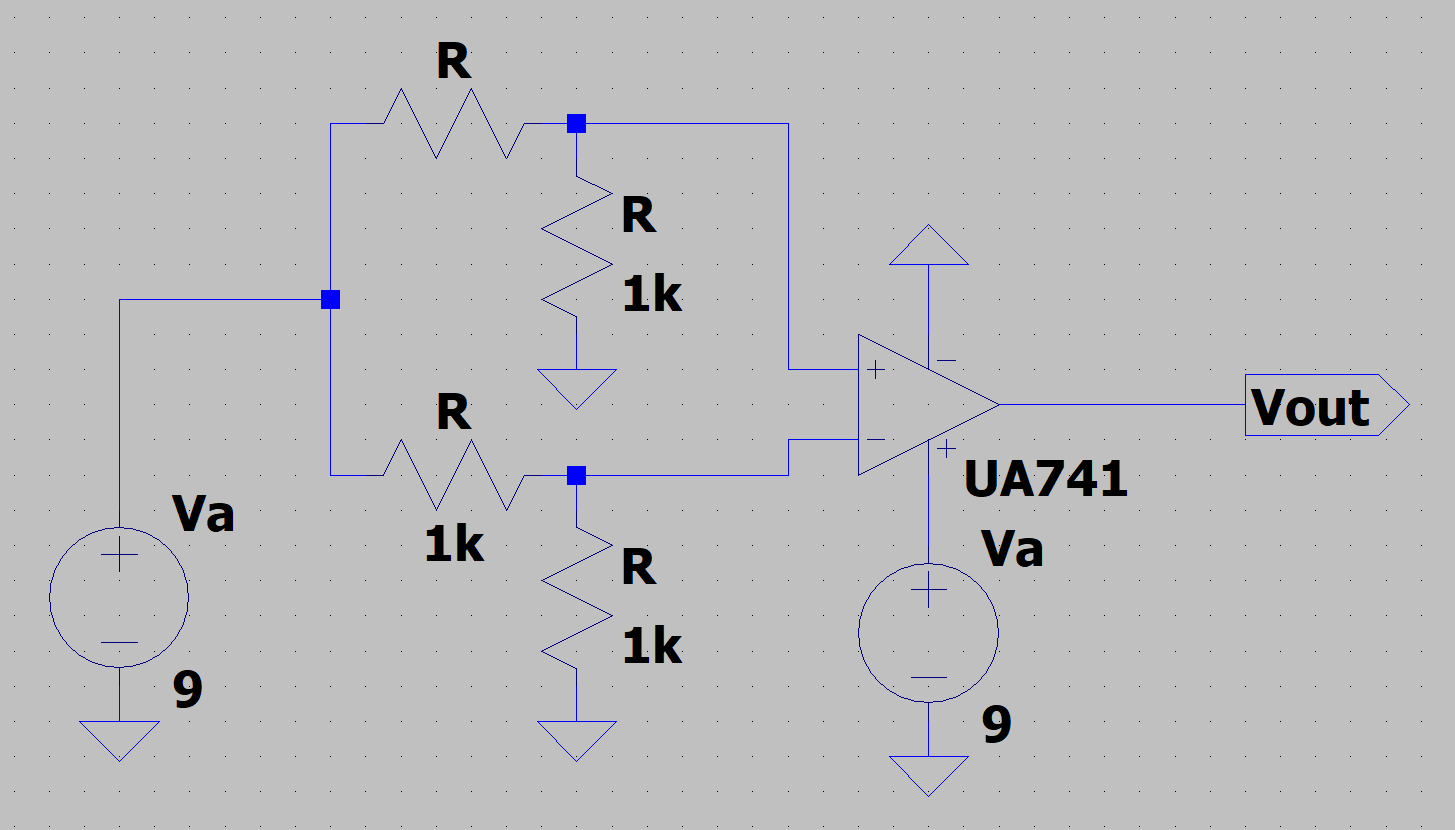
\includegraphics[height=6.9cm]{immagini/dimNTC}
	\caption{Schema della rete del termistore NTC dimensionata.} 
	\label{figura:dimNTC}
\end{figure}
Nella figura \ref{figura:NTCout} vengono invece mostrati i grafici che si ottengono in uscita all'amplificatore operazionale quando il circuito si trova nello stato di allarme ($T = \SI{40}{\celsius}$; $R_T=\SI{617}{\ohm}$) e di riposo ($T = \SI{10}{\celsius}$; $R_T=\SI{1.70}{k\ohm}$). Vediamo che il comportamento del circuito è quello che ci aspettiamo. \par
\begin{figure}[h!]
	\centering
	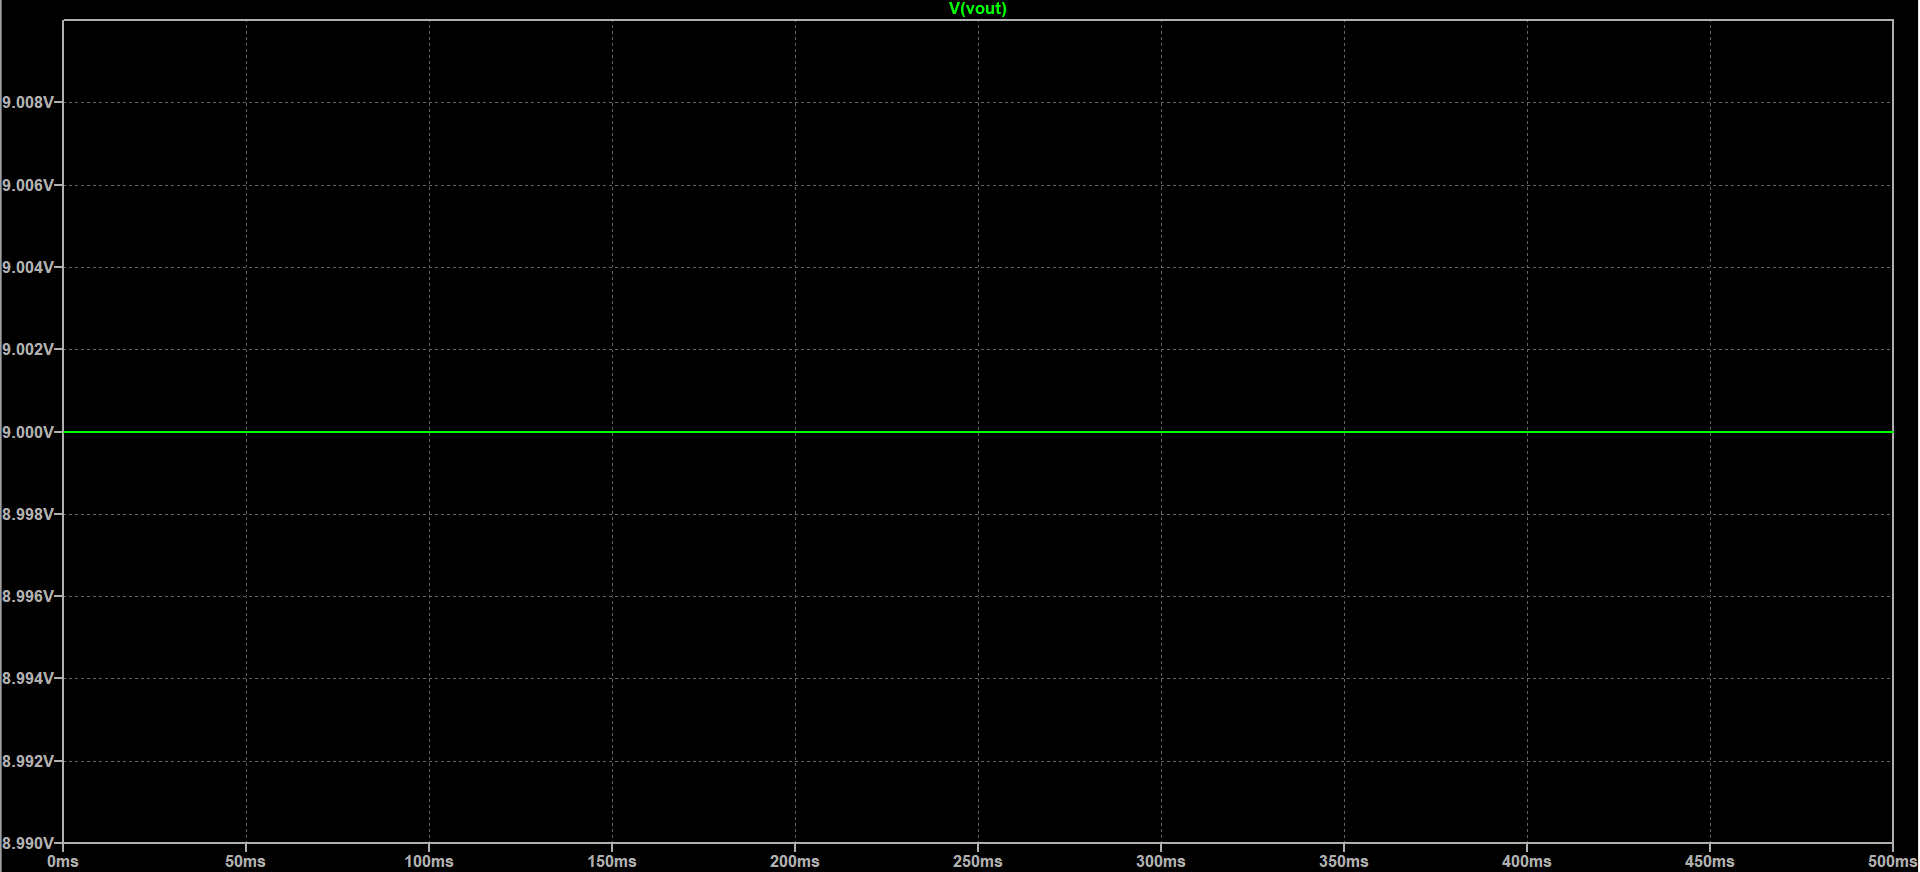
\includegraphics[height=6cm]{immagini/NTCon}
	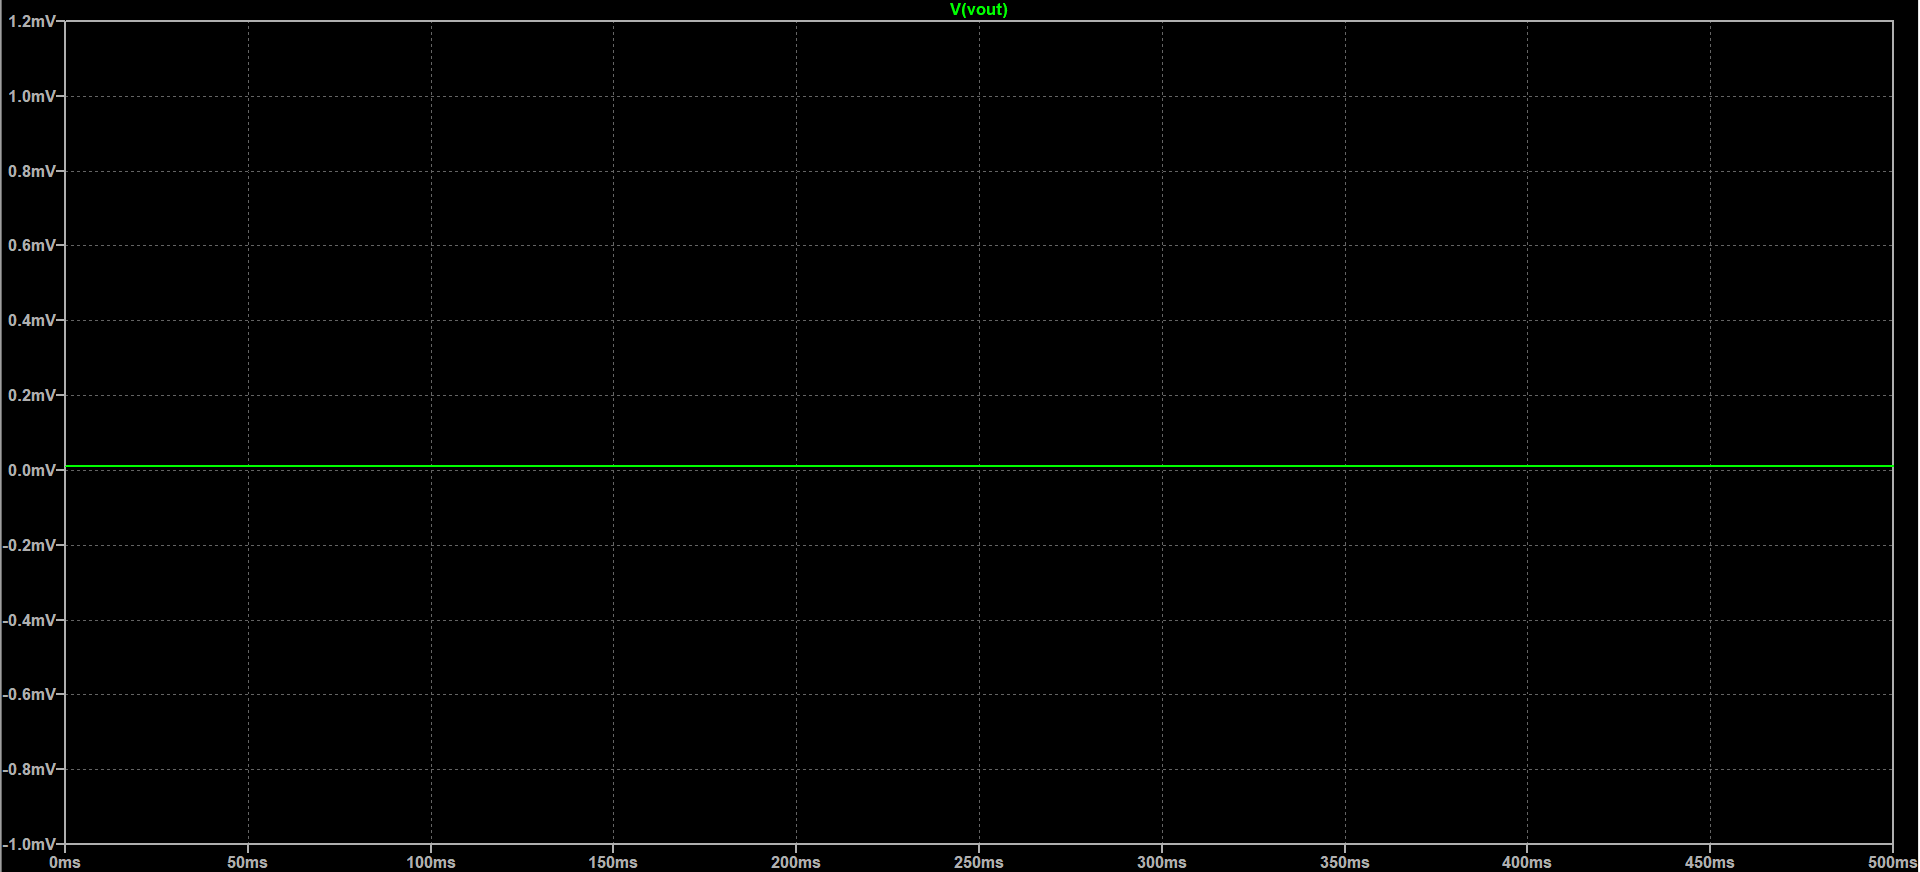
\includegraphics[height=6cm]{immagini/NTCoff}
	\caption{Grafico dell'uscita quando il sistema è nello stato di allarme (sopra) e riposo (sotto).} 
	\label{figura:NTCout}
\end{figure}

\newpage
\section{Simulazione del circuito}
Prima di simulare il circuito, dobbiamo integrare i due sottosistemi. Per come sono stati progettati, è sufficiente collegare l'uscita dell'OPAMP al pin 4 del timer 555, senza utilizzare altri componenti dato che entrambi i componenti lavorano con le stesse tensioni. Il circuito complessivo è rappresentato in figura \ref{figura:schemaFinale}.
\begin{figure}[h!]
	\centering
	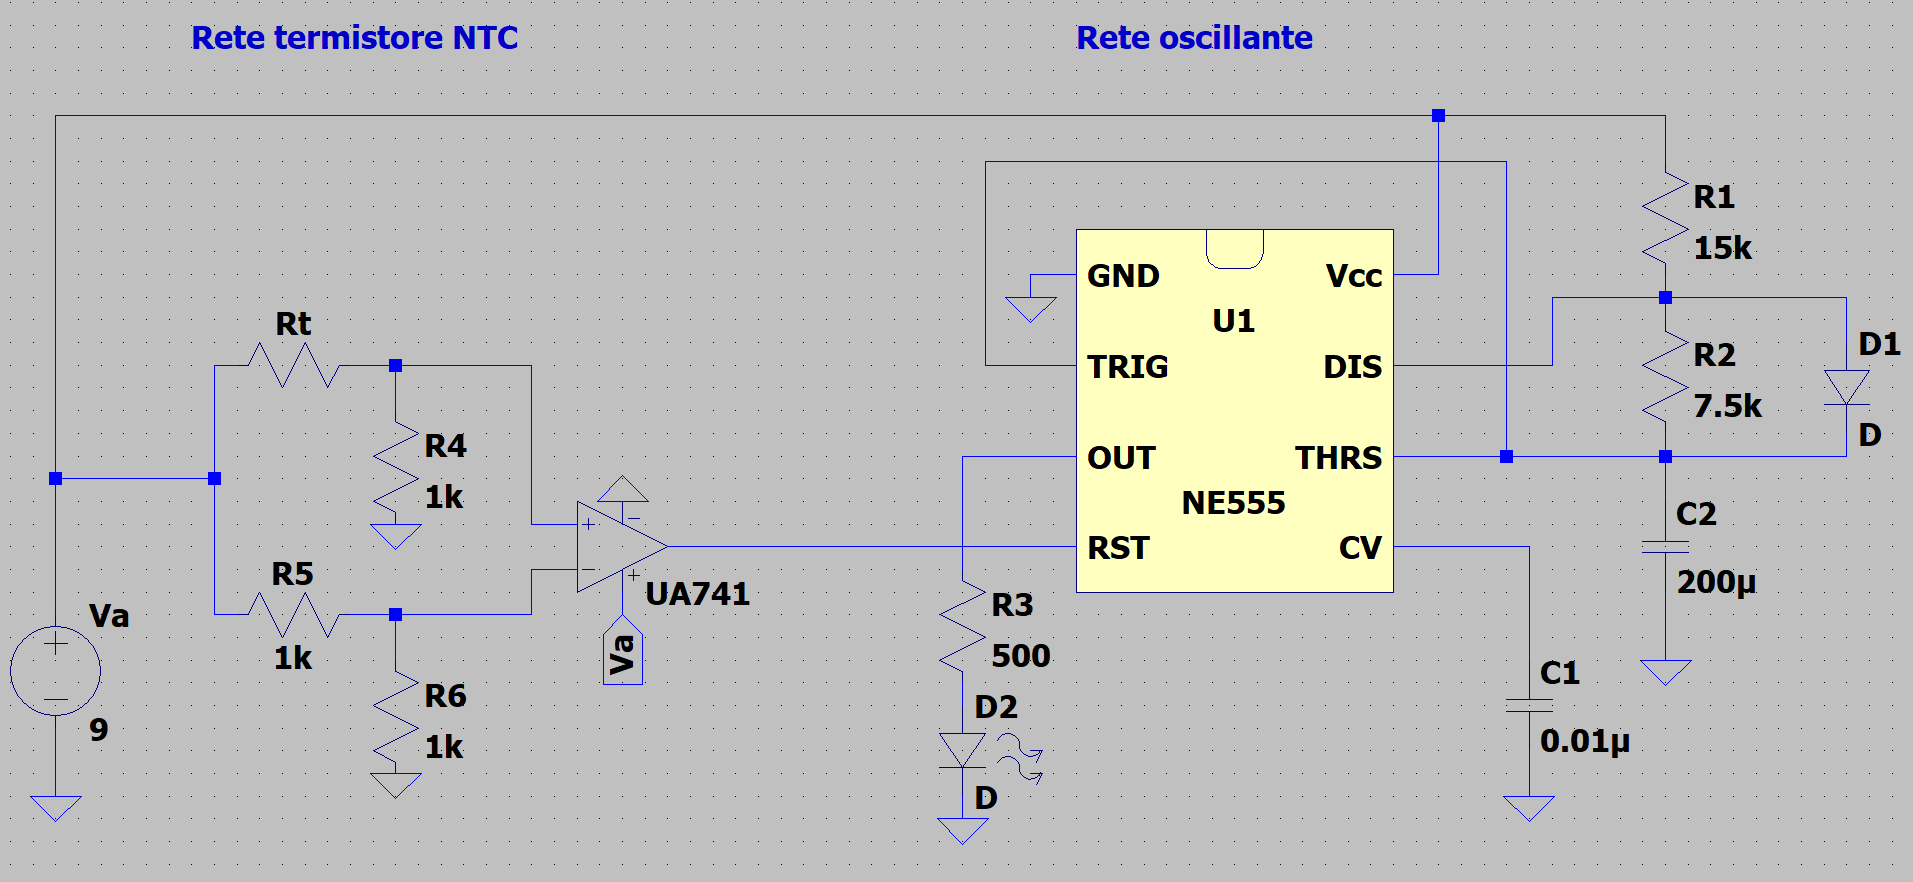
\includegraphics[width=\textwidth]{immagini/schemaFinale}
	\caption{Schema del circuito finale.} 
	\label{figura:schemaFinale}
\end{figure}
\\Una volta ottenuto il circuito complessivo, per verificarne il corretto funzionamento lo abbiamo simulato utilizzando due programmi differenti: \textit{LTSpice} e \textit{Tinkercad}.  
\subsection{Simulazione con LTSpice}
Per la simulazione con \textit{LTSpice} utilizziamo il circuito mostrato in figura \ref{figura:schemaFinale}. Vediamo prima come si comporta il sistema quando è nello stato di allarme, perciò con $R_T$ che vale \SI{617}{\ohm}. Si riporta di seguito il grafico con il confronto della tensione in uscita all'amplificatore operazionale (che coincide con la tensione applicata al pin 4 del timer 555) e la tensione misurata ai capi del LED. Successivamente, simuliamo il circuito quando non si trova nello stato di allarme, dunque con $R_T$ che vale \SI{1.70}{k\ohm}. Questi grafici sono riportati nelle figure \ref{figura:sistemaON} e \ref{figura:sistemaOFF}. \par
\begin{figure}[h!]
	\centering
	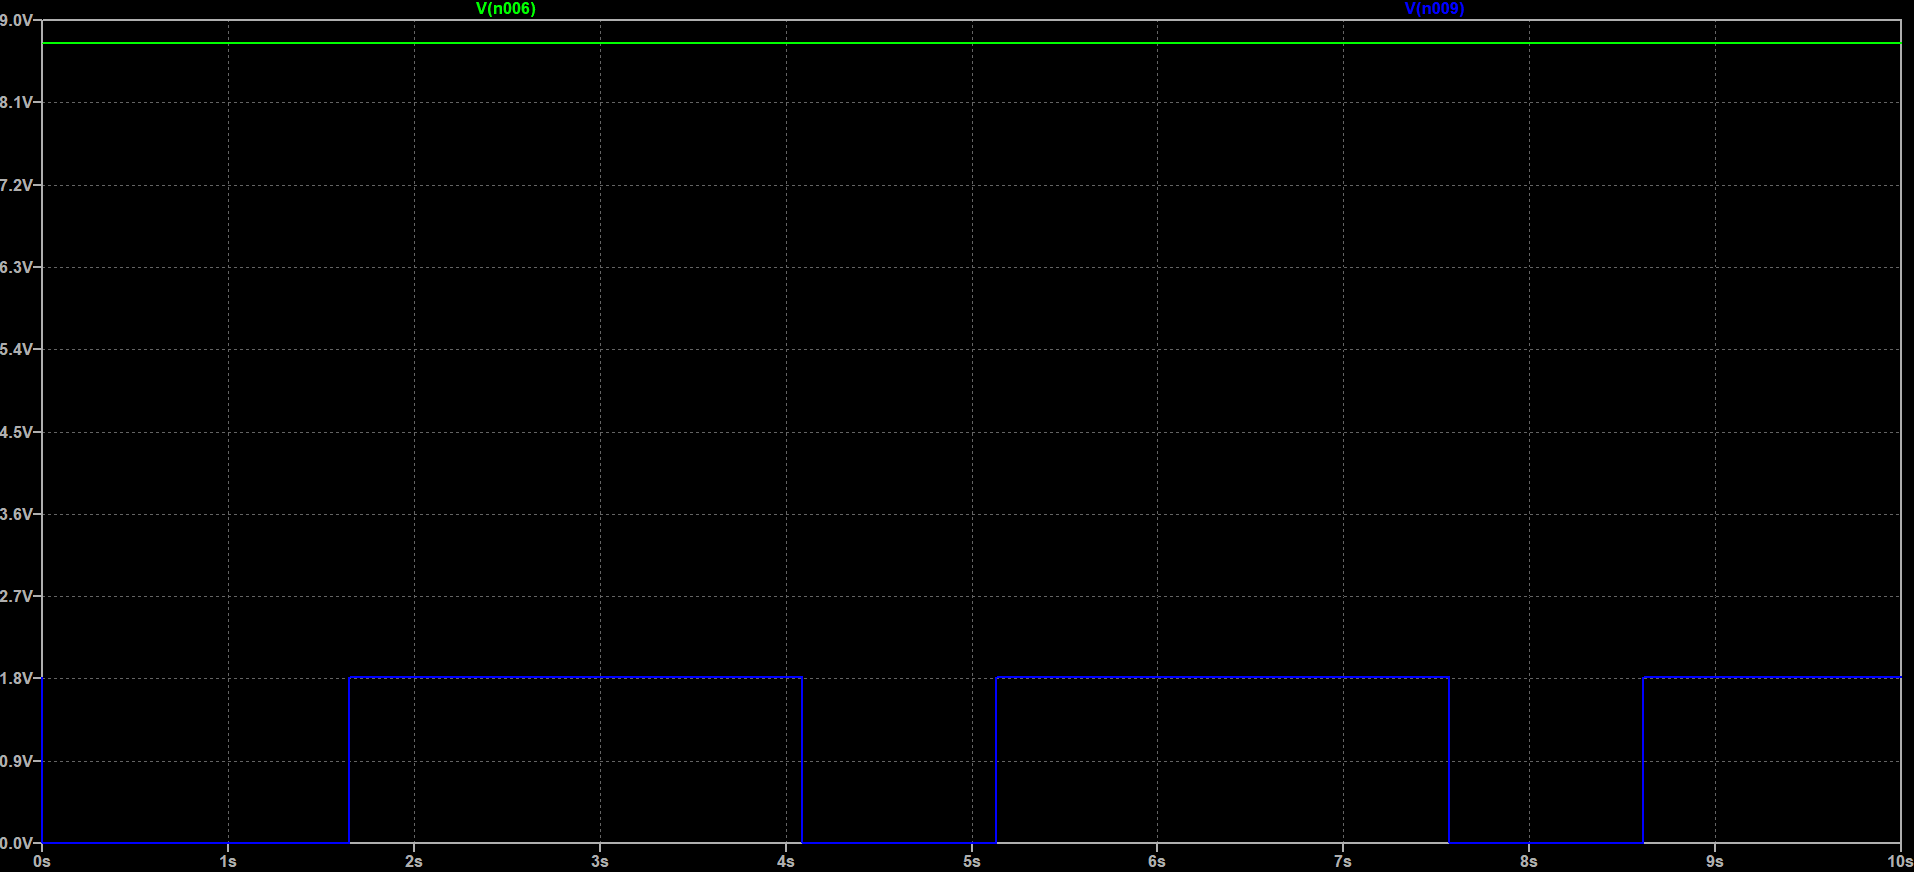
\includegraphics[width=\textwidth]{immagini/sistemaON}
	\caption{Uscita del circuito quando si trova nello stato di allarme.} 
	\label{figura:sistemaON}
\end{figure}
\begin{figure}[h!]
	\centering
	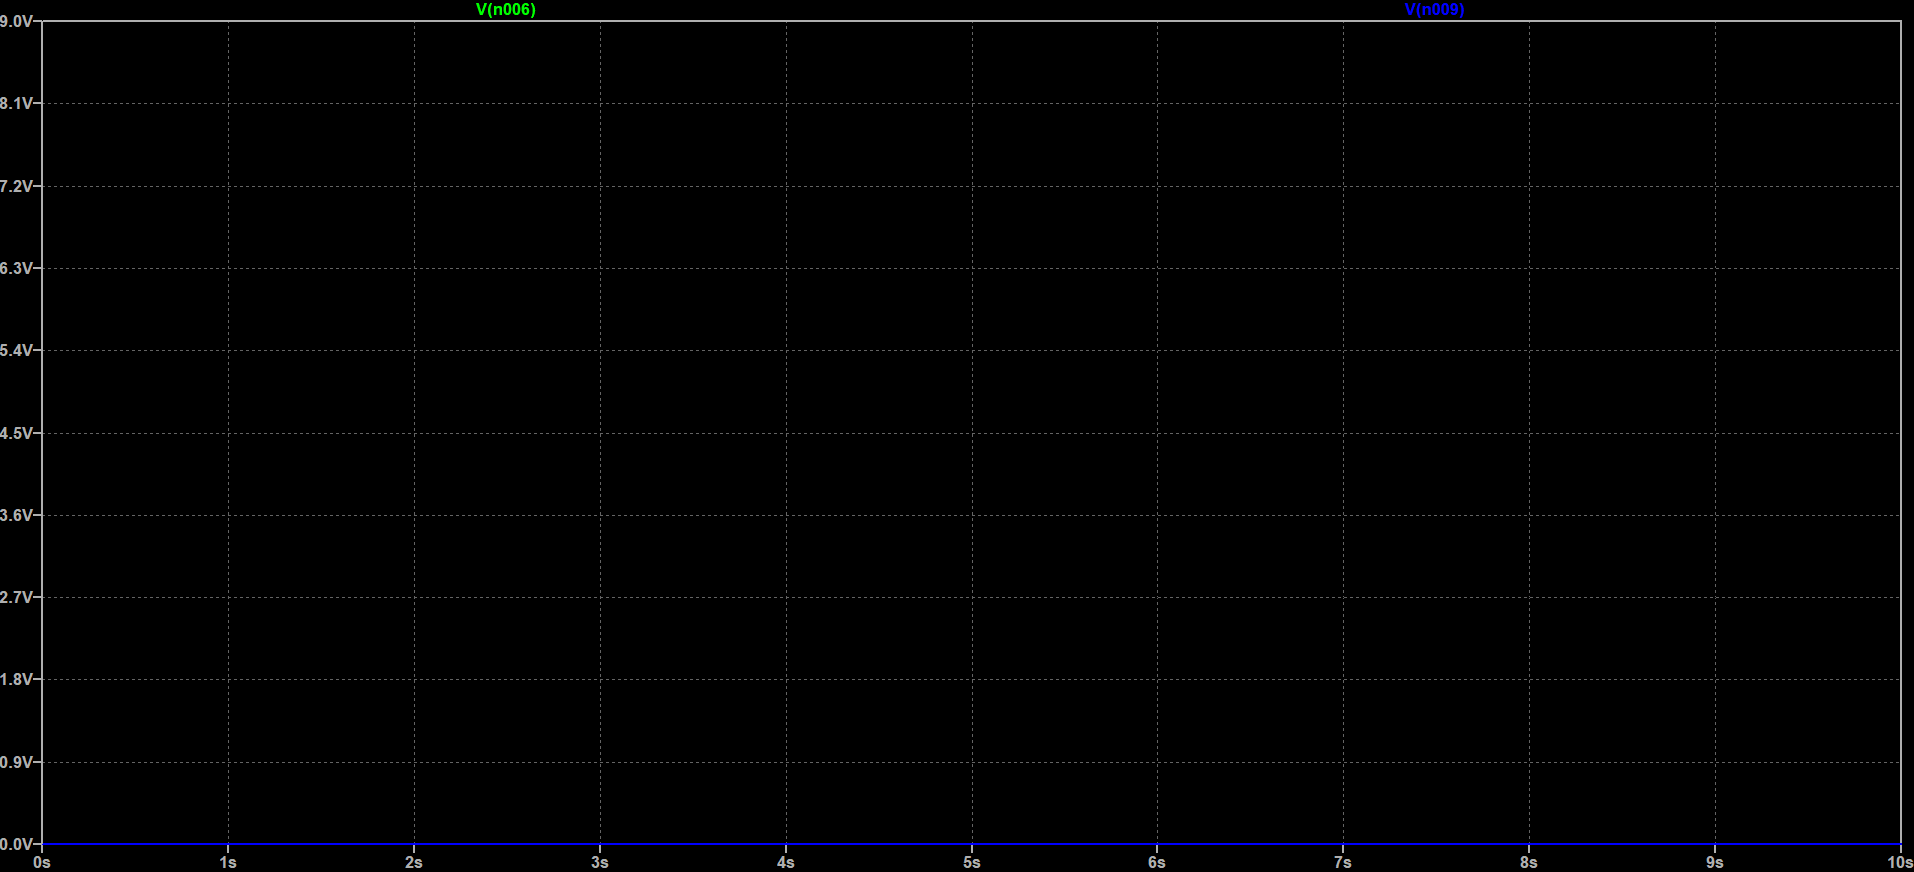
\includegraphics[width=\textwidth]{immagini/sistemaOFF}
	\caption{Uscita del circuito quando non si trova nello stato di allarme.} 
	\label{figura:sistemaOFF}
\end{figure}
Per entrambe le figure, la traccia verde corrisponde all'uscita dell'OPAMP, mentre quella blu alla tensione ai capi del diodo. Possiamo osservare che il comportamento del circuito è corretto, perché produce l'onda quadra solo quando il termistore registra una temperatura superiore a T = \SI{25}{\celsius}. \par
Per simulare meglio le transizioni tra i due stati, utilizzeremo un altro programma, \textit{Tinkercad}. I risultati di questa simulazione sono descritti nella sezione successiva (sezione \ref{tinkercad}). 

\subsection{Simulazione con Tinkercad}\label{tinkercad}
Per quanto riguarda la simulazione in \textit{Tinkercad}, per prima cosa abbiamo realizzato il circuito della figura \ref{figura:schemaFinale} su una breadboard. Per poter costruire il circuito (come in figura \ref{figura:tinkercad_breadboard}) sono stati inseriti i componenti dimensionati come specificato nella sezione precedente, ma è stata apportata una variazione: è stato cambiato il sensore di temperatura e in particolare è stato utilizzato un potenziometro di valore \SI{2}{\kilo\ohm} al posto del termistore NTC.

\begin{figure}[h!]
	\centering
	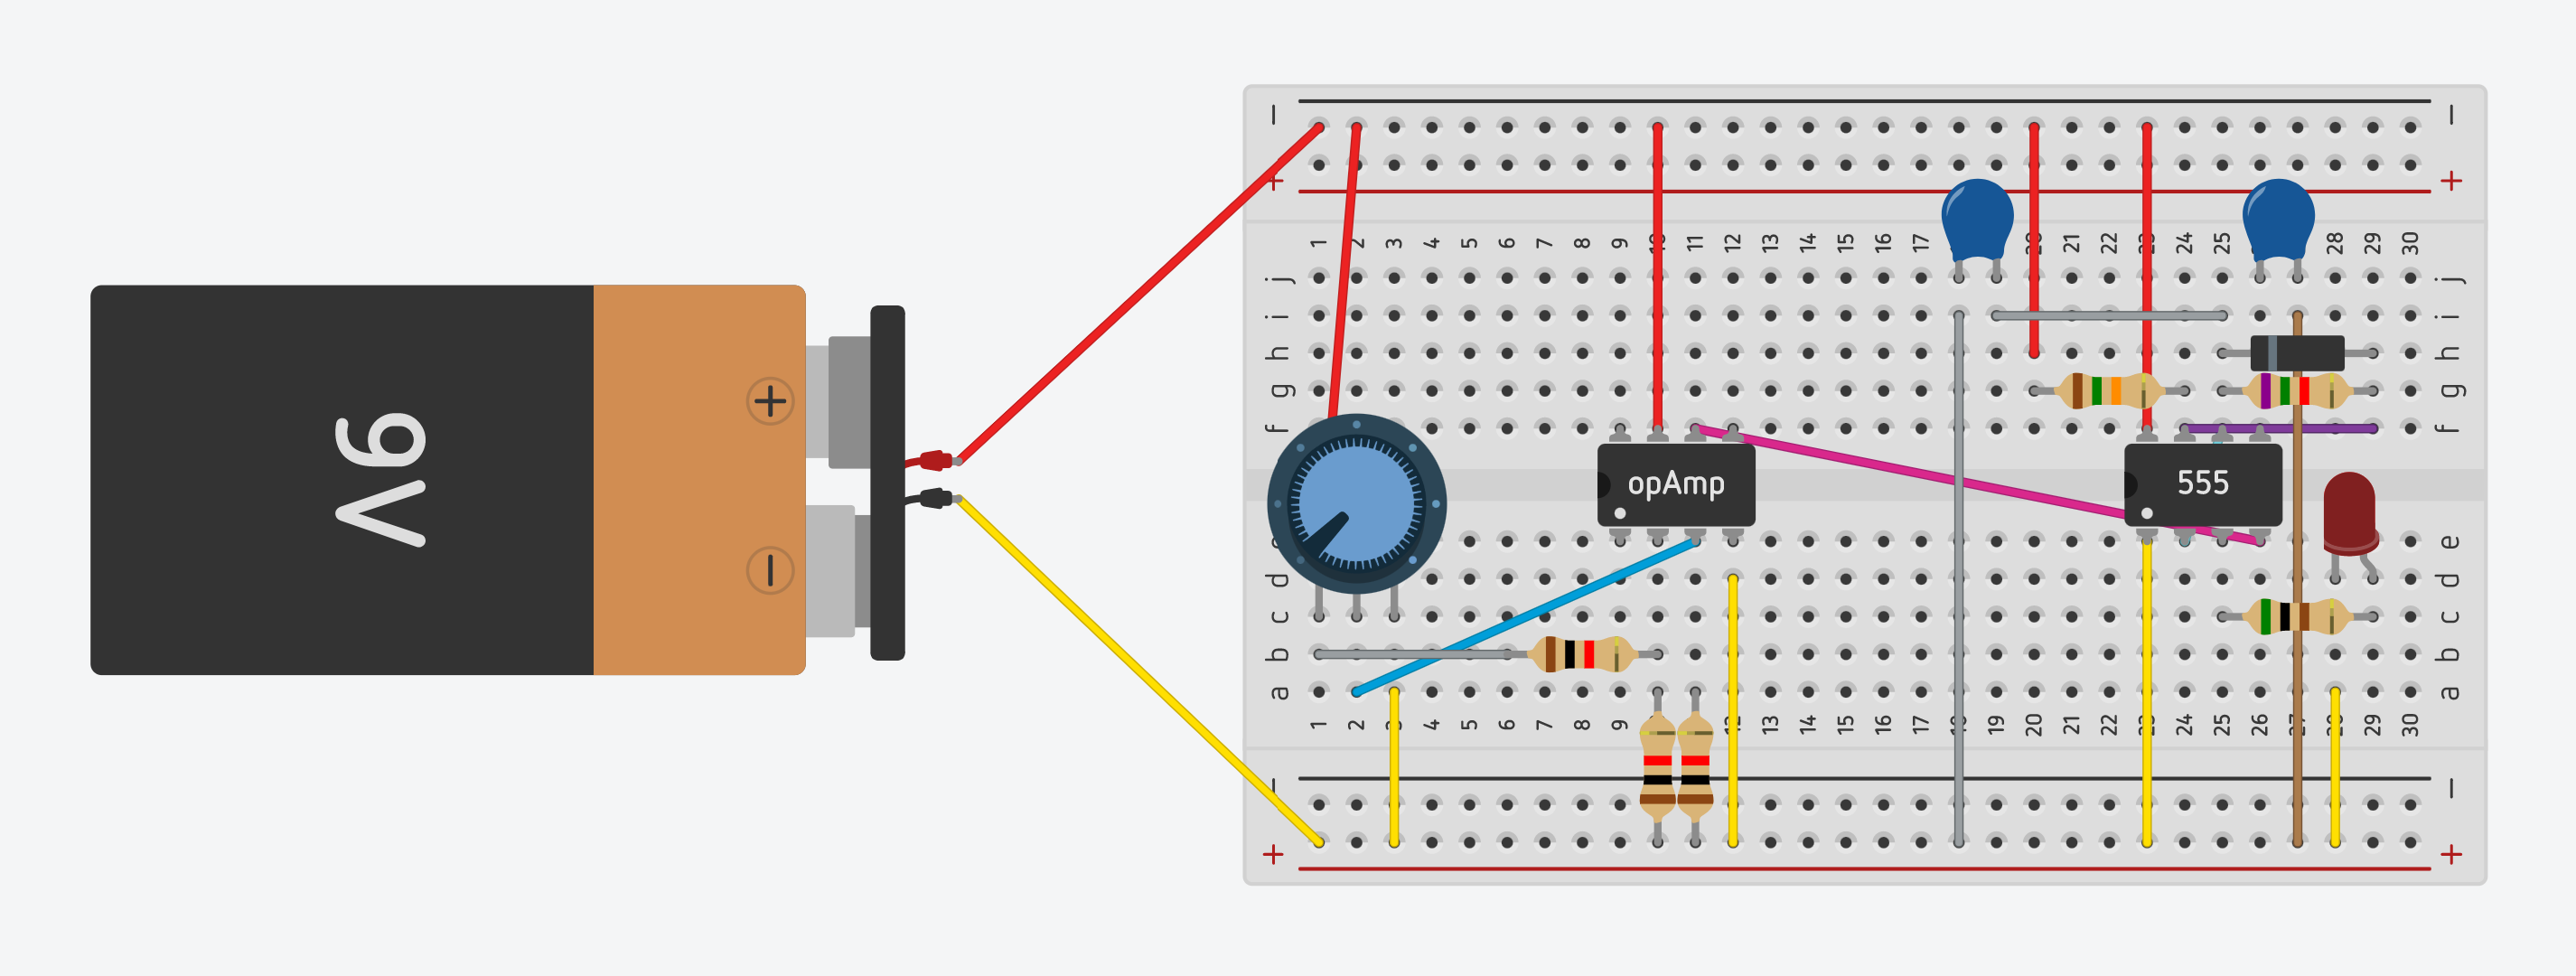
\includegraphics[height=6cm]{immagini/tinkercad_breadboard}
	\caption{Breadboard su cui è stato realizzato il circuito in \textit{Tinkercad}.} 
	\label{figura:tinkercad_breadboard}
\end{figure}

Poi per verificare il comportamento del sistema rispetto ai risultati ottenuti con \textit{LTSpice}, abbiamo simulato il circuito (\textcolor{blue}{\underline{\href{https://www.tinkercad.com/things/5cgEecbtMyg-copy-of-stunning-snicket/editel?sharecode=9z73QqFvXyHOBVZMRfgNmmMNsfyYwwq-TDywLOMkaKc}{simulazione}}}).

\noindent La prima simulazione effettuata considera un valore di temperatura maggiore di \SI{25}{\celsius} e quindi ci si trova in stato di allarme siccome il valore del potenziometro $R_T$ è inferiore a \SI{1}{\kilo\ohm}. In questo caso il valore di \SI{617}{\ohm} associato ad $R_T$ è stato approssimato a \SI{600}{\ohm} in modo da poterlo definire con la manopola del potenziometro (valore determinato dalla misura effettuata con un multimetro). In questa condizione la manopola del potenziometro deve essere rivolta verso sinistra.

Invece la seconda simulazione eseguita è caratterizzata da un valore di temperatura minore di \SI{25}{\celsius} e di conseguenza non ci si trova nello stato di allarme perchè il potenziometro $R_T$ assume un valore maggiore di \SI{1}{\kilo\ohm}. In quest'altro caso il valore di \SI{1.70}{\kilo\ohm} associato ad $R_T$ è stato approssimato a \SI{1.68}{\kilo\ohm} in modo da poterlo definire con la manopola del potenziometro (valore determinato dalla misura effettuata con un multimetro). In questa condizione la manopola del potenziometro deve essere rivolta verso destra.

I segnali dell'uscita dell'OPAMP (oscilloscopio con i fili verdi) e della tensione ai capi del LED (oscilloscopio con i fili blu) ottenuti per le precedenti due condizioni analizzate sono stati riportati nelle figure \ref{figura:tinkercad_on} e \ref{figura:tinkercad_off} rispettivamente.

\begin{figure}[h!]
	\centering
	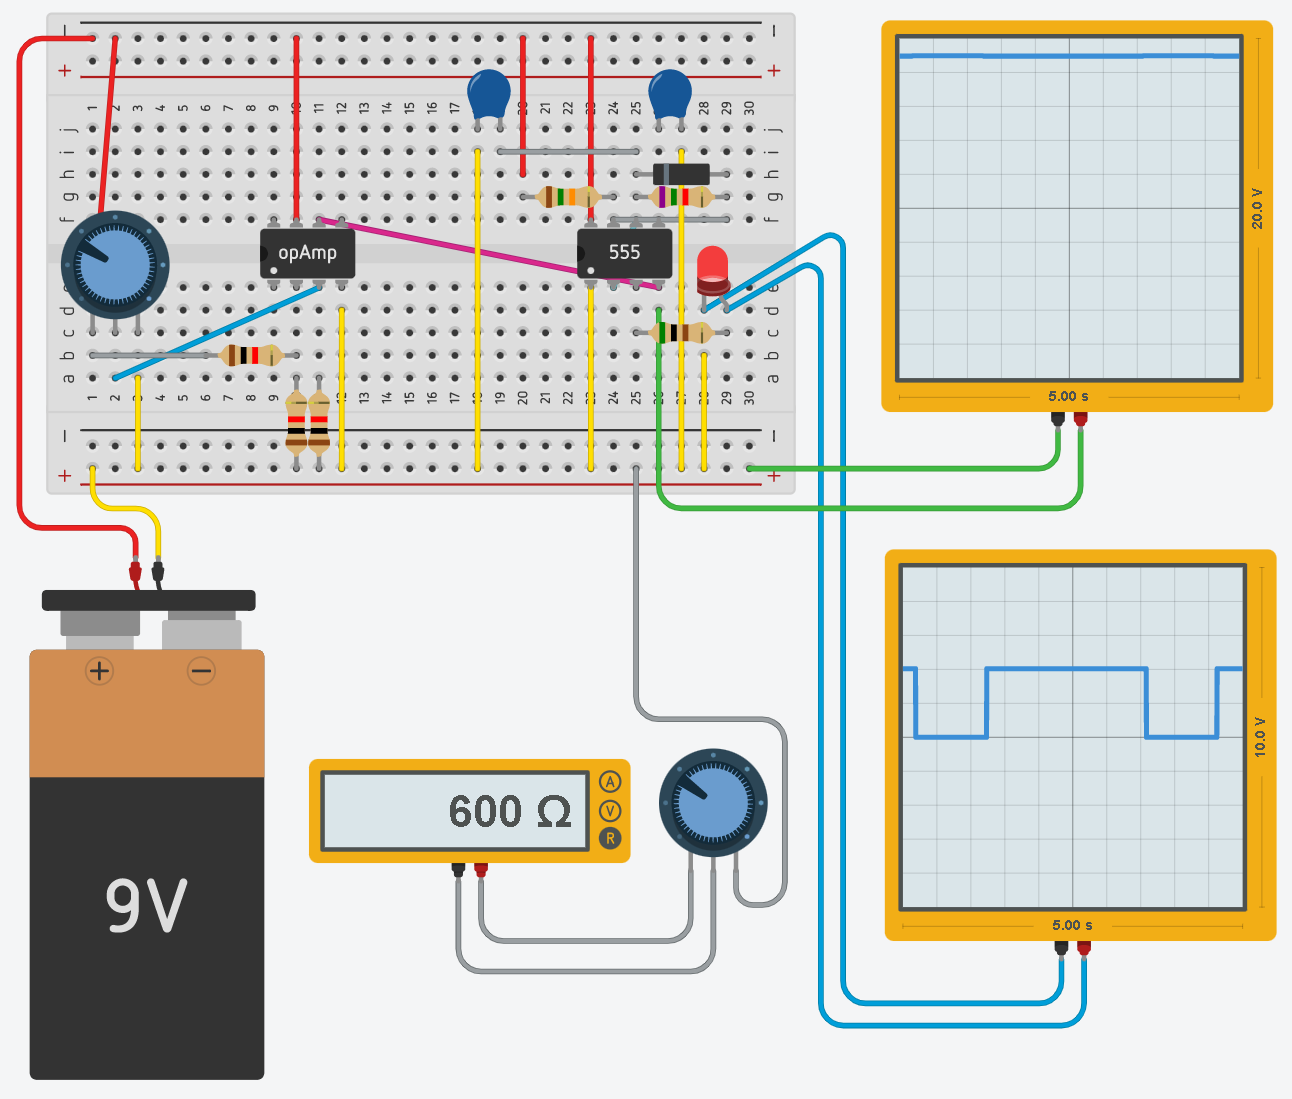
\includegraphics[width=\textwidth]{immagini/tinkercad_on}
	\caption{Simulazione del circuito quando si trova nello stato di allarme.} 
	\label{figura:tinkercad_on}
\end{figure}

\begin{figure}[h!]
	\centering
	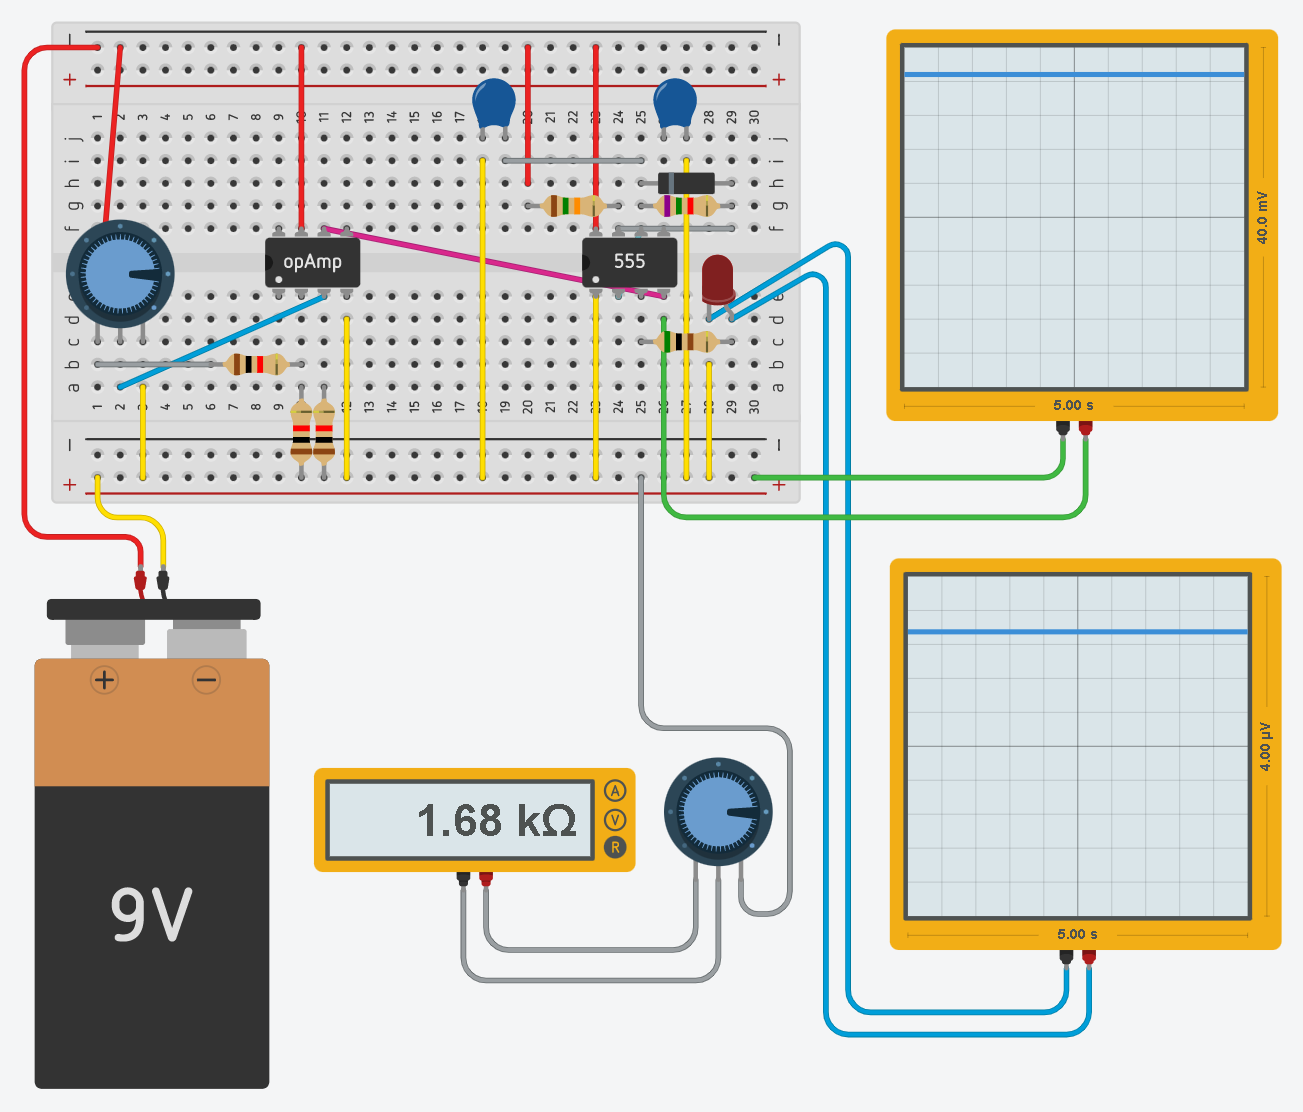
\includegraphics[width=\textwidth]{immagini/tinkercad_off}
	\caption{Simulazione del circuito quando non si trova nello stato di allarme.} 
	\label{figura:tinkercad_off}
\end{figure}

Dalle immagini di queste simulazioni si può notare che si ottiene il comportamento desiderato, che era stato descritto nella precedente sezione: quando la temperatura supera i \SI{25}{\celsius} l'allarme è attivo e difatti il segnale della tensione ai capi del LED corrisponde a un'onda quadra, mentre quando si ha una temperatura inferiore l'allarme è spento e di conseguenza il segnale della tensione sul diodo è sempre prossima a 0. 

\end{document}